\documentclass{article}

\usepackage{graphicx}
\usepackage{tikz}
\usepackage{tikzsymbols}
\usetikzlibrary{calc,patterns,shapes.geometric}
\pagestyle{empty}
\usepackage[margin=0pt]{geometry}
\geometry{papersize={14in,12in}}

\def\centerarc[#1](#2)(#3:#4:#5){\draw[#1] ($(#2)+({#5*cos(#3)},{#5*sin(#3)})$) arc (#3:#4:#5);}

\begin{document}
	\begin{figure}
		\centering
		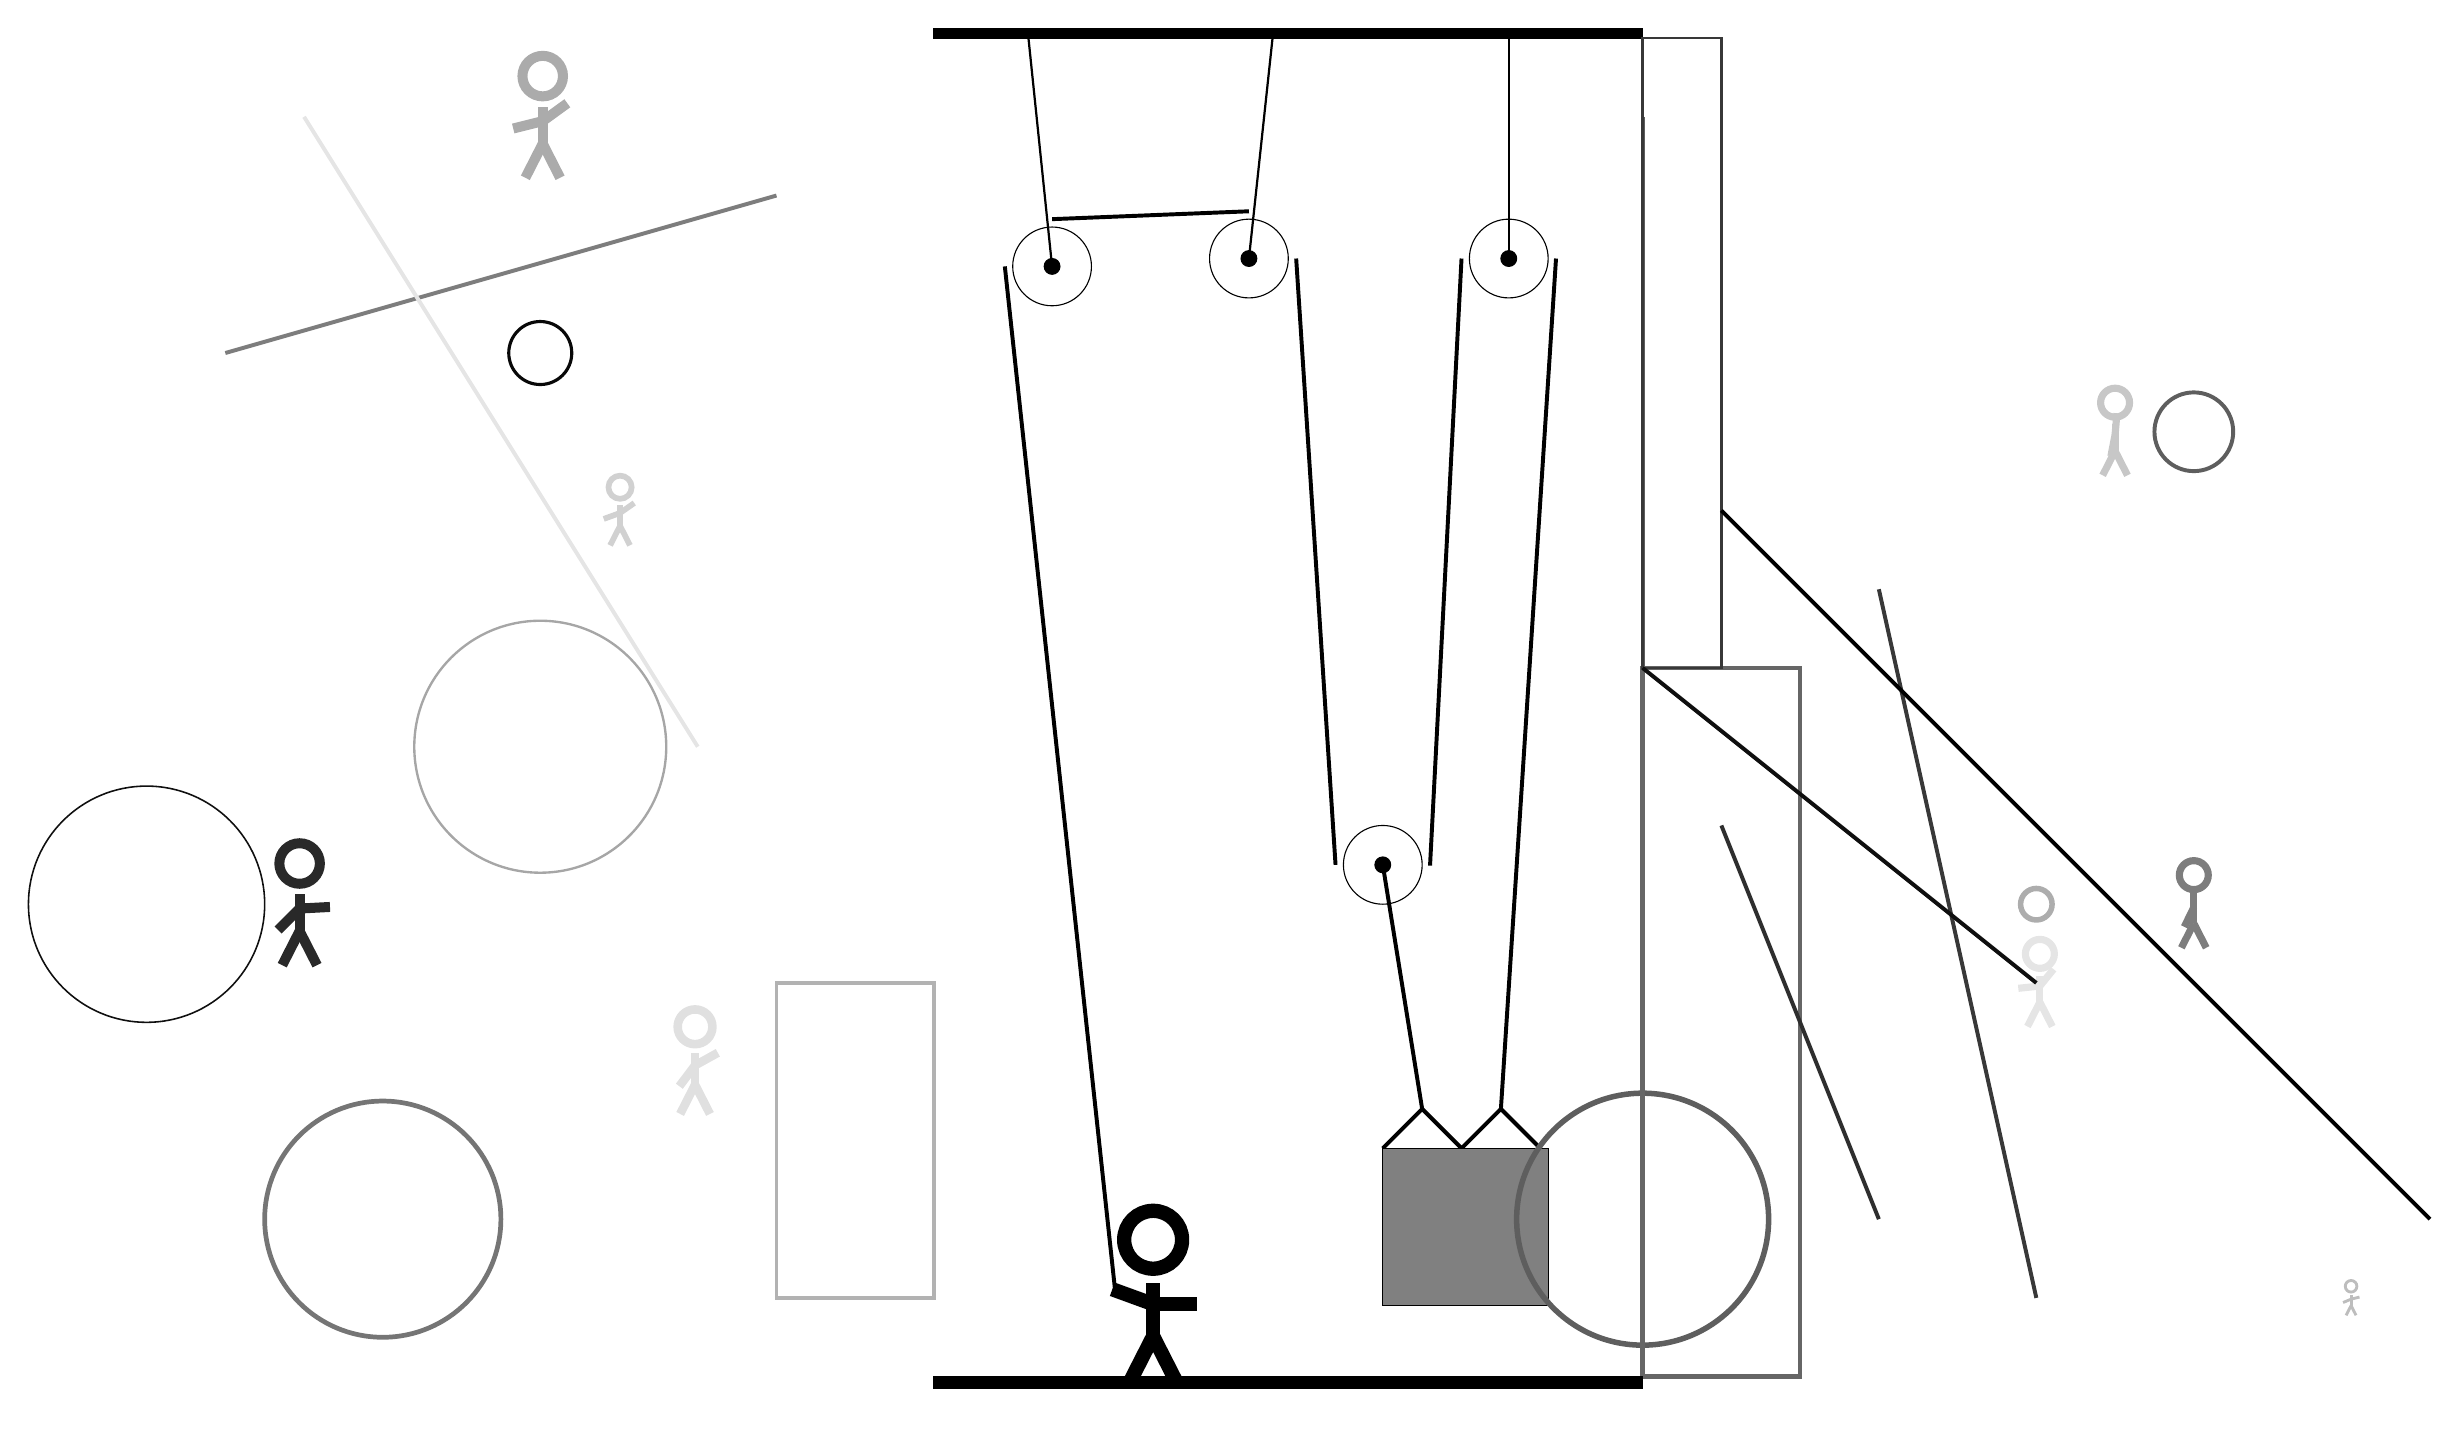
\begin{tikzpicture}
			%%%%% START %%%%%
			
			\draw[fill=black] (-3, 14) rectangle (6, 14.125);
			
			\draw (1, 11.2) circle (0.5);
			\draw[fill=black] (1, 11.2) circle (0.1);
			\draw[thick] (1, 11.2) -- (1.3, 14);
			
			\draw (4.3, 11.2) circle (0.5);
			\draw[fill=black] (4.3, 11.2) circle (0.1);
			\draw[thick] (4.3, 11.2) -- (4.3, 14);
			
			\draw (2.7, 3.5) circle (0.5);
			\draw[fill=black] (2.7, 3.5) circle (0.1);
			
			\draw[line width=0.5mm]  (2.7, -0.1) -- (3.2, 0.4) -- (3.7, -0.1) -- (4.2, 0.4) -- (4.7, -0.1);
			\draw[fill=black!50] (2.7, -0.1) rectangle (4.8, -2.1);
			
			\draw [line width=0.7mm, color=black!32](11, 3) circle (0.2);
			
			\draw [line width=0.2mm, color=black!94](-13, 3) circle (1.5);
			\draw [line width=0.5mm, color=black!63](13, 9) circle (0.5);
			\node[line width=0.5mm, color=black!33] at (-8, 13) {\Strichmaxerl[7][14][36]};
			\draw[line width=0.6mm, color=black!52] (-5, 10) rectangle (-5, 10);
			\draw[line width=0.5mm, color=black!78](11, -2) -- (9, 7);
			
			\node[line width=0.7mm, color=black!18] at (-7, 8) {\Strichmaxerl[4][20][35]};
			\draw[line width=0.5mm, color=black!63](6, 13) -- (6, -2);
			\node[line width=0.2mm, color=black!12] at (-6, 1) {\Strichmaxerl[6][53][29]};
			\draw [line width=0.7mm, color=black!63](6, -1) circle (1.6);
			\node[line width=0.7mm, color=black!26] at (15, -2) {\Strichmaxerl[2][23][14]};
			\node[line width=0.2mm, color=black!10] at (11, 2) {\Strichmaxerl[5][6][51]};
			\draw[line width=0.6mm, color=black!60] (6, -3) rectangle (8, 6);
			
			\draw [line width=0.3mm, color=black!35](-8, 5) circle (1.6);
			\draw[line width=0.3mm, color=black!78] (6, 6) rectangle (7, 14);
			\draw[line width=0.5mm, color=black!51](-5, 12) -- (-12, 10);
			
			\node[line width=0.7mm, color=black!51] at (13, 3) {\Strichmaxerl[5][64][90]};
			\draw[line width=0.5mm, color=black!100](7, 8) -- (16, -1);
			\draw[line width=0.5mm, color=black!10](-6, 5) -- (-11, 13);
			\draw[line width=0.5mm, color=black!82](7, 4) -- (9, -1);
			\draw[line width=0.5mm, color=black!94](11, 2) -- (6, 6);
			\node[line width=0.5mm, color=black!84] at (-11, 3) {\Strichmaxerl[7][45][3]};
			
			\draw [line width=0.4mm, color=black!97](-8, 10) circle (0.4);
			\draw [line width=0.6mm, color=black!54](-10, -1) circle (1.5);
			\draw[line width=0.5mm, color=black!30] (-5, -2) rectangle (-3, 2);
			
			\node[line width=0.5mm, color=black!22] at (12, 9) {\Strichmaxerl[5][79][85]};
			
			\draw (-1.5, 11.1) circle (0.5);
			\draw[fill=black] (-1.5, 11.1) circle (0.1);
			\draw[thick] (-1.5, 11.1) -- (-1.8, 14);
			
			\draw[line width=0.5mm](-0.7, -1.9) --  (-2.1, 11.1);
			\centerarc[line width=0.5mm](-1.5, 11.1)(90:180:0.6);
			\draw[line width=0.5mm](-1.5, 11.7) -- (1, 11.8);
			\centerarc[line width=0.5mm](1, 11.2)(0:90:0.6);
			\draw[line width=0.5mm](1.6, 11.2) -- (2.1, 3.5);
			\centerarc[line width=0.5mm](2.7, 3.5)(180:370:0.6);
			\draw[line width=0.5mm] (3.3, 3.49) -- (3.7, 11.2);
			\centerarc[line width=0.5mm](4.3, 11.2)(0:180:0.6);
			\draw[line width=0.5mm](4.2, 0.4) -- (4.9, 11.2);
			\draw[line width=0.5mm] (3.2, 0.4) -- (2.7, 3.5);
			
			\node at (-0.2, -2) {\Strichmaxerl[10][-20][0]};
			
			\draw[fill=black] (-3, -3) rectangle (6, -3.15);
			
			%%%%% END %%%%%
		\end{tikzpicture}
	\end{figure}	
\end{document}